\newpage
\section{Coupling growing rootsystems to numerical models} \label{sec:growing}

    
\subsection{Mapping of growing roots and underlying soil} 

\lstinputlisting[firstline=1, language=Python, caption=Example 7a]{../../examples/python/example7a_mapping.py}

\begin{itemize}
\item[46-49] aaa
\end{itemize}

\subsection{Coupling a dynamic root system to DuMux with soil feedback} \label{sec:dumux_dyn_coupling}

We modify Example \ref{sec:dumux_coupling}. Using the class MappedRootSystem (as before) it is sufficient to call MappedRootSystem::simulate() to implement real root growth, i.e. to add rs.simulate(dt) in L80. The modified segments and the mapping of new segments is automatically managed (see example7b\_coupling.py).


In this example soil state does not affect root system growth in any way. We need to add the processes we are interested in (see Section \ref{sec:tropism} and \ref{sec:functional}). For demonstration how to do that, we demonstrate the implementation steps using hydrotropim. Note that the other interactions from Section \\ref{sec:functional} could be implemented in the same way. 

In order to use hydrotropism, we need to define a SoilLookUp that accesses the dynamic soil data. We present two appraoches: the first uses nearest neighbour interpolation, which is fast but a coarse approximation. The second uses linear interpolation which is more exact, but slower. 

\lstinputlisting[firstline=1, language=Python, caption=Example 7c]{../../examples/python/example7c_feedback.py}


\begin{itemize}
\item[46-49] aaa
\end{itemize}

Figure \ref{fig:example7c} shows that hydrotropism will lead to increased cumulative uptake, because the roots are more evenly distributed. Note that there is a big variation in the results, and for a more profound analysis we would have to make many simualtion runs. 

\begin{figure}
\begin{subfigure}[c]{1\textwidth}
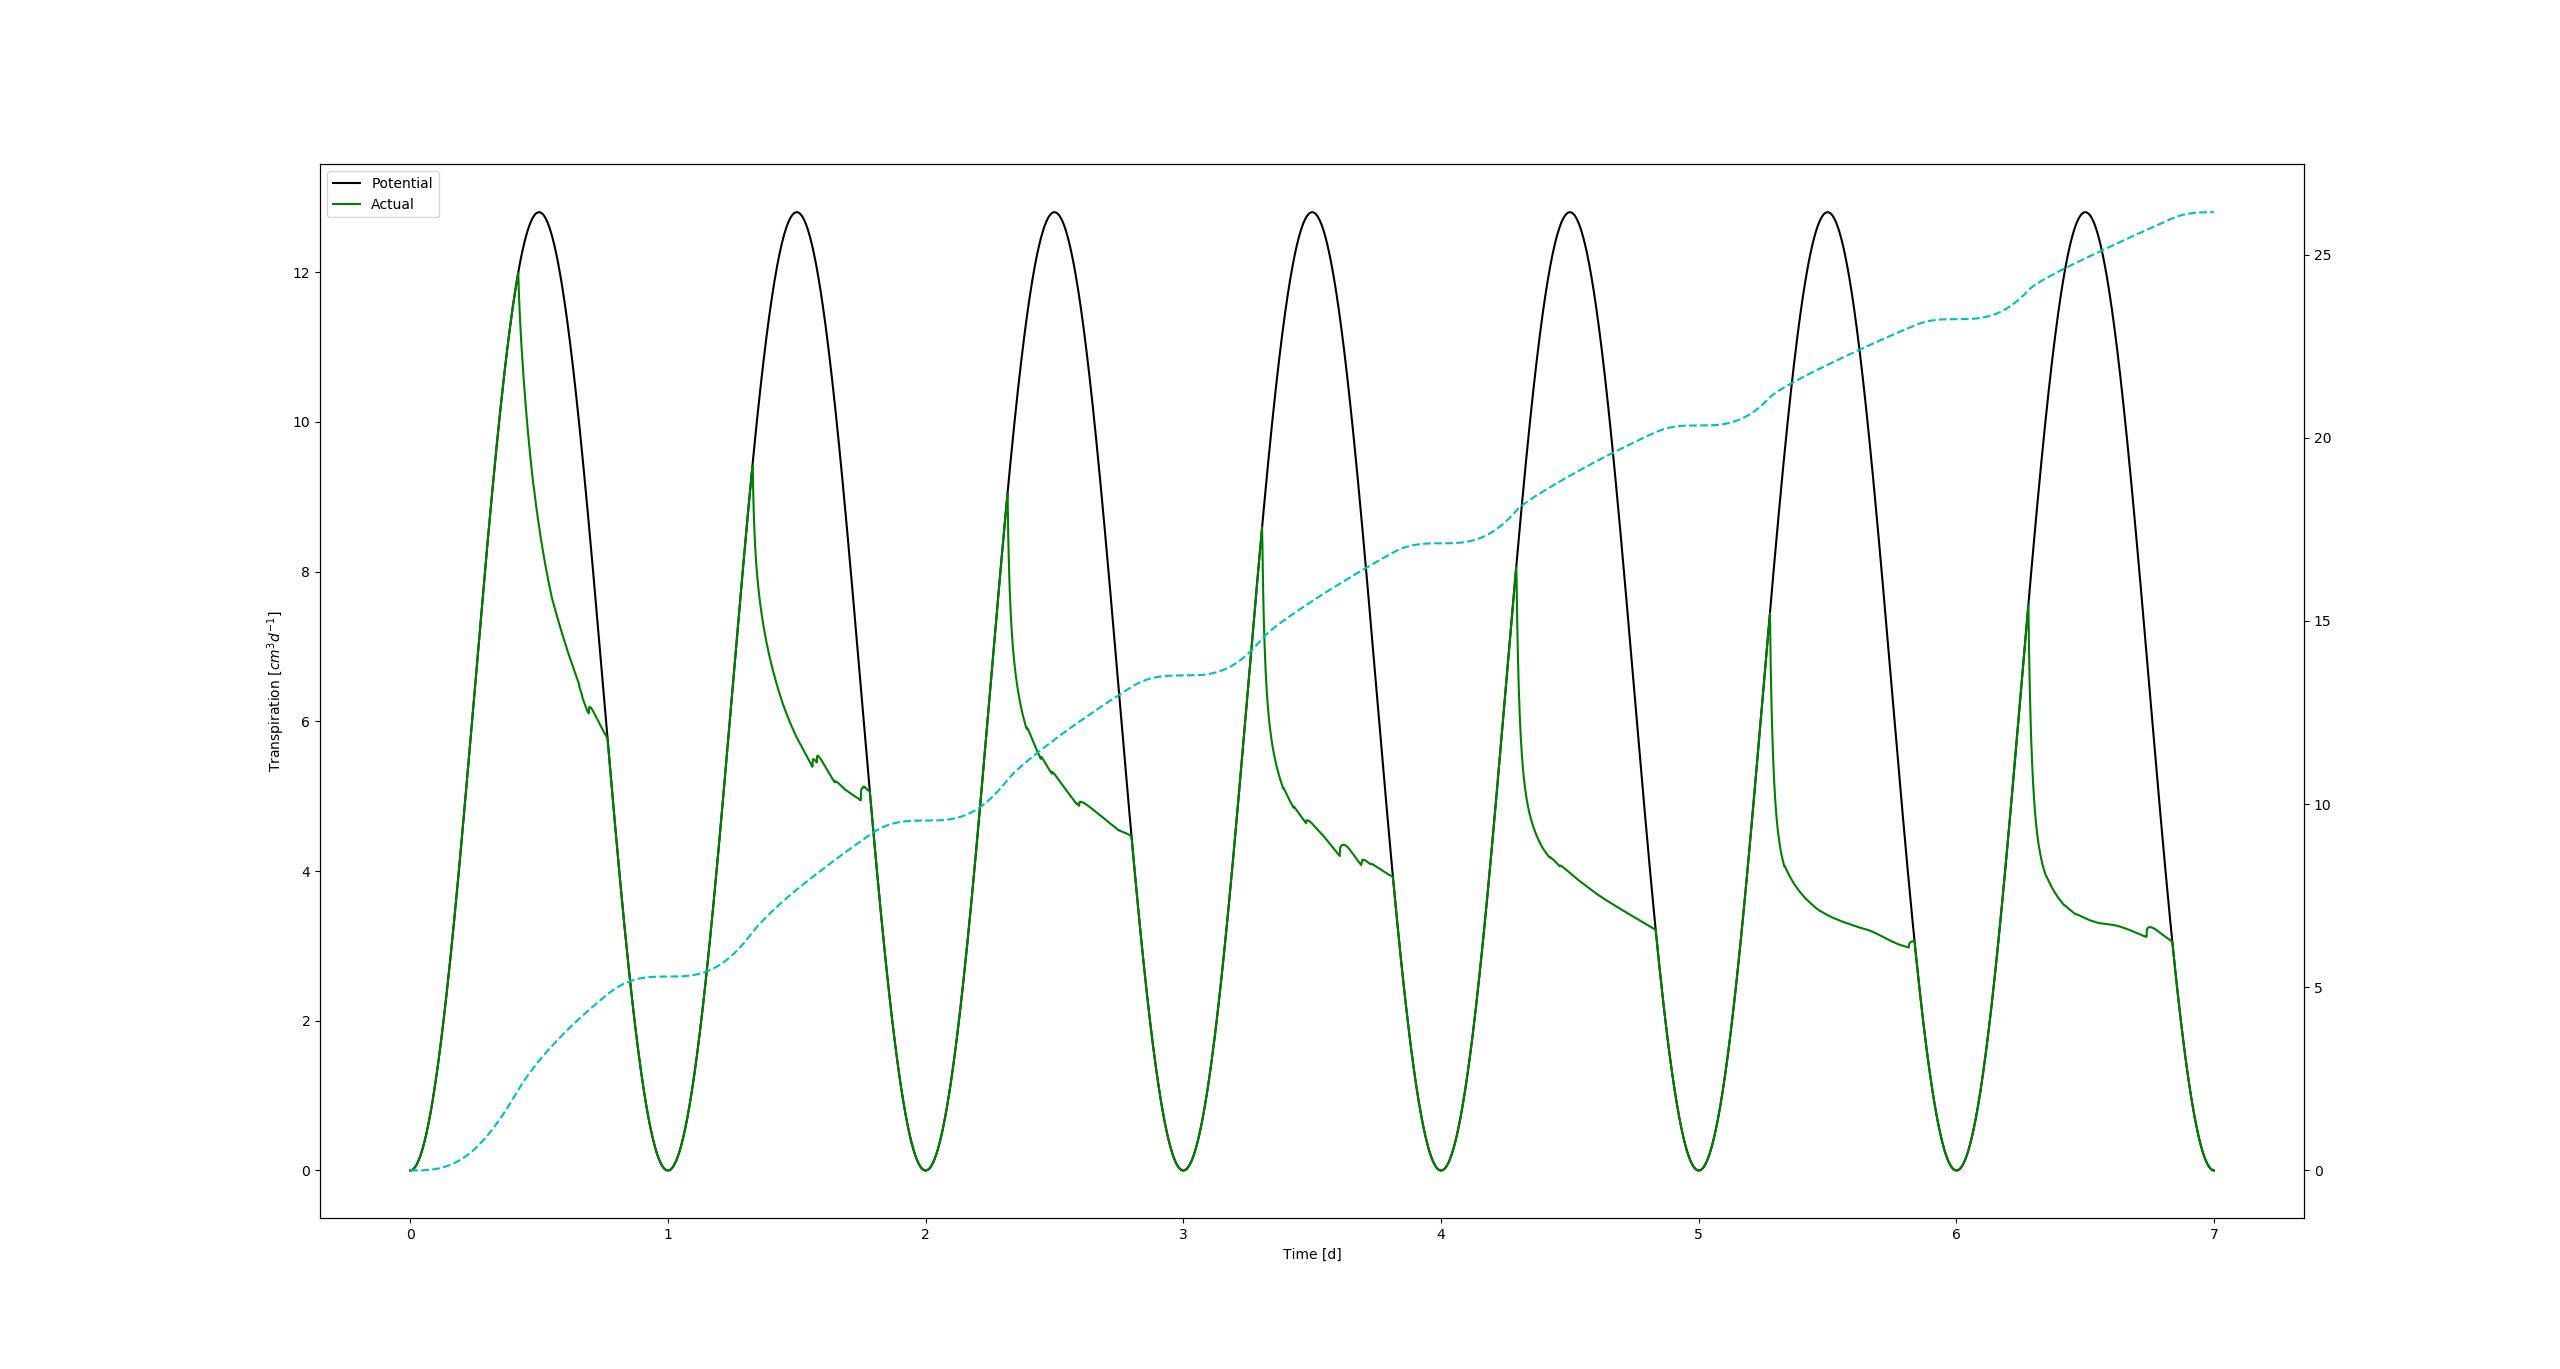
\includegraphics[width=0.99\textwidth]{example7c_no_hydro.png}
\subcaption{Gravi- and Plagiotropism} \label{fig:example7c}
\end{subfigure}
\begin{subfigure}[c]{1\textwidth}
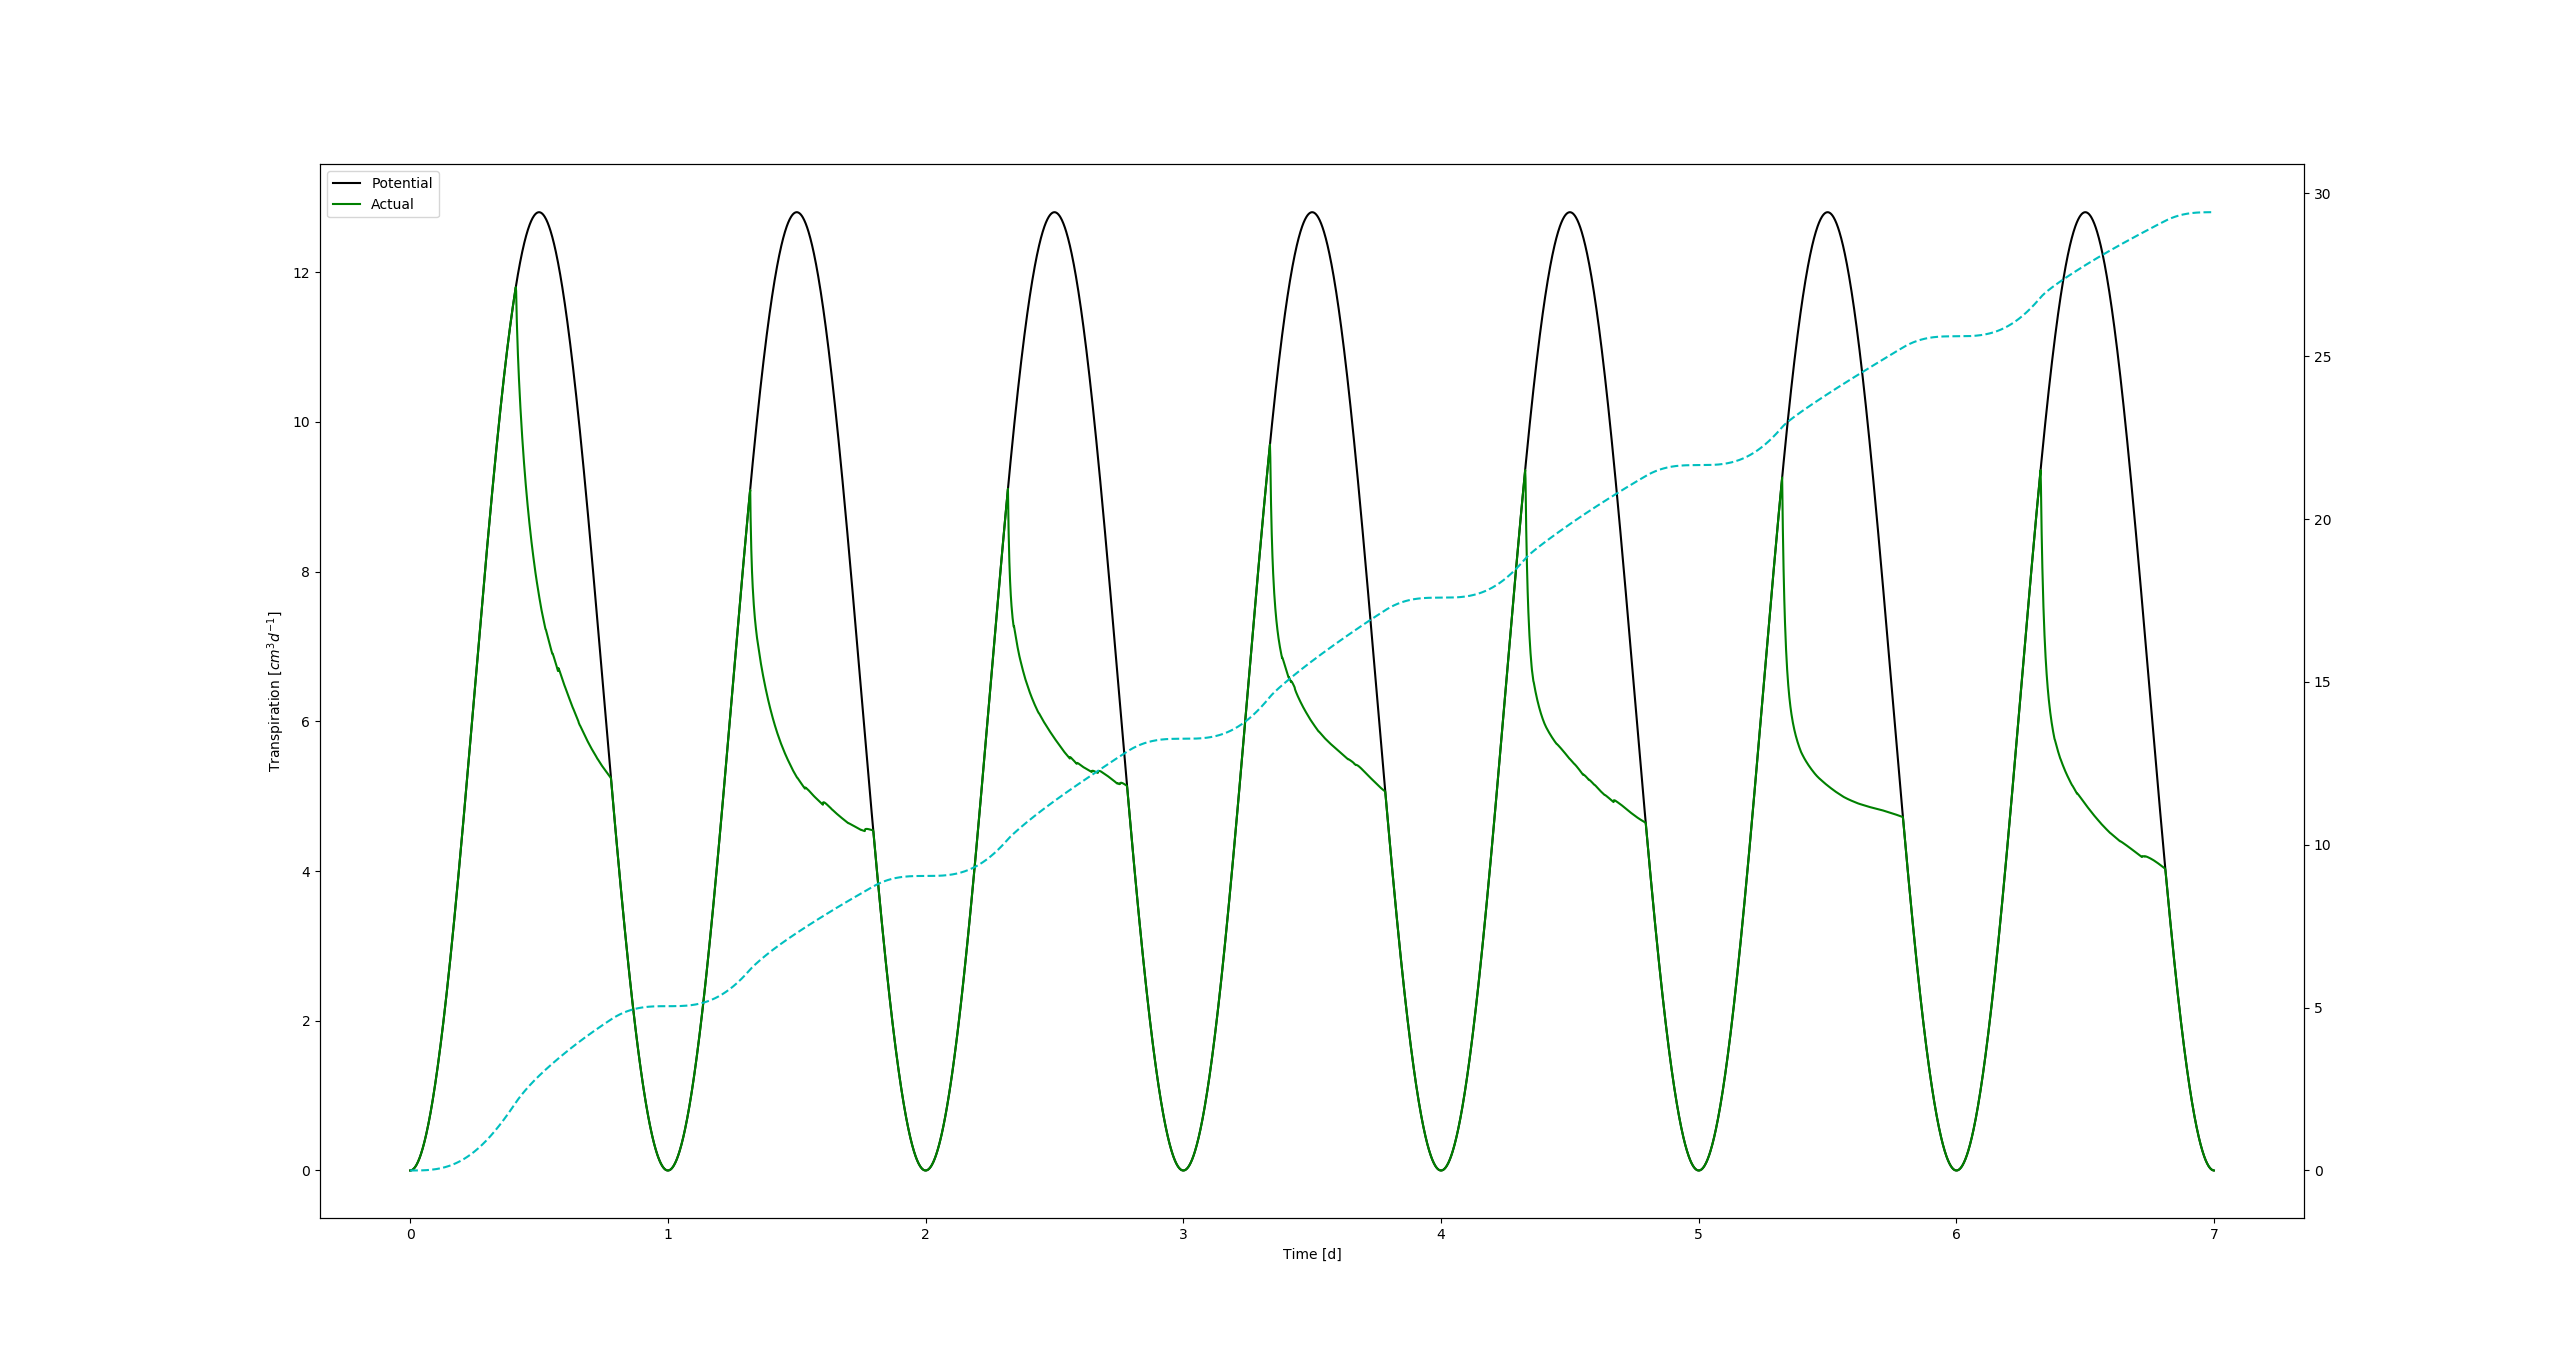
\includegraphics[width=0.99\textwidth]{example7c_simple_hydro.png}
\subcaption{Hydrotropism} \label{fig:example7c_hydro}
\end{subfigure}
\caption{Water uptake a in plant pot} \label{fig:example7c}
\end{figure}







\newpage
\section{Todos}
Topics that are not covered yet or should be improved

\begin{itemize}

\item The DuMux binding and MPI

\item Elongation rate according to Moacir et al.

\item Delay based, versus length based lateral emergance.

\item Better branching probability example.

\item Periodicity without DuMux coupling, but with a soil 3d grid (untested, and an example is missing)

\item Carbon limited root system growth

\end{itemize}

